\section{Introduction}
\label{sec:intro}

% \begin{figure}[tb]
% 	\centering
% 	\begin{subfigure}{0.49\linewidth}
% 		\centering
% 		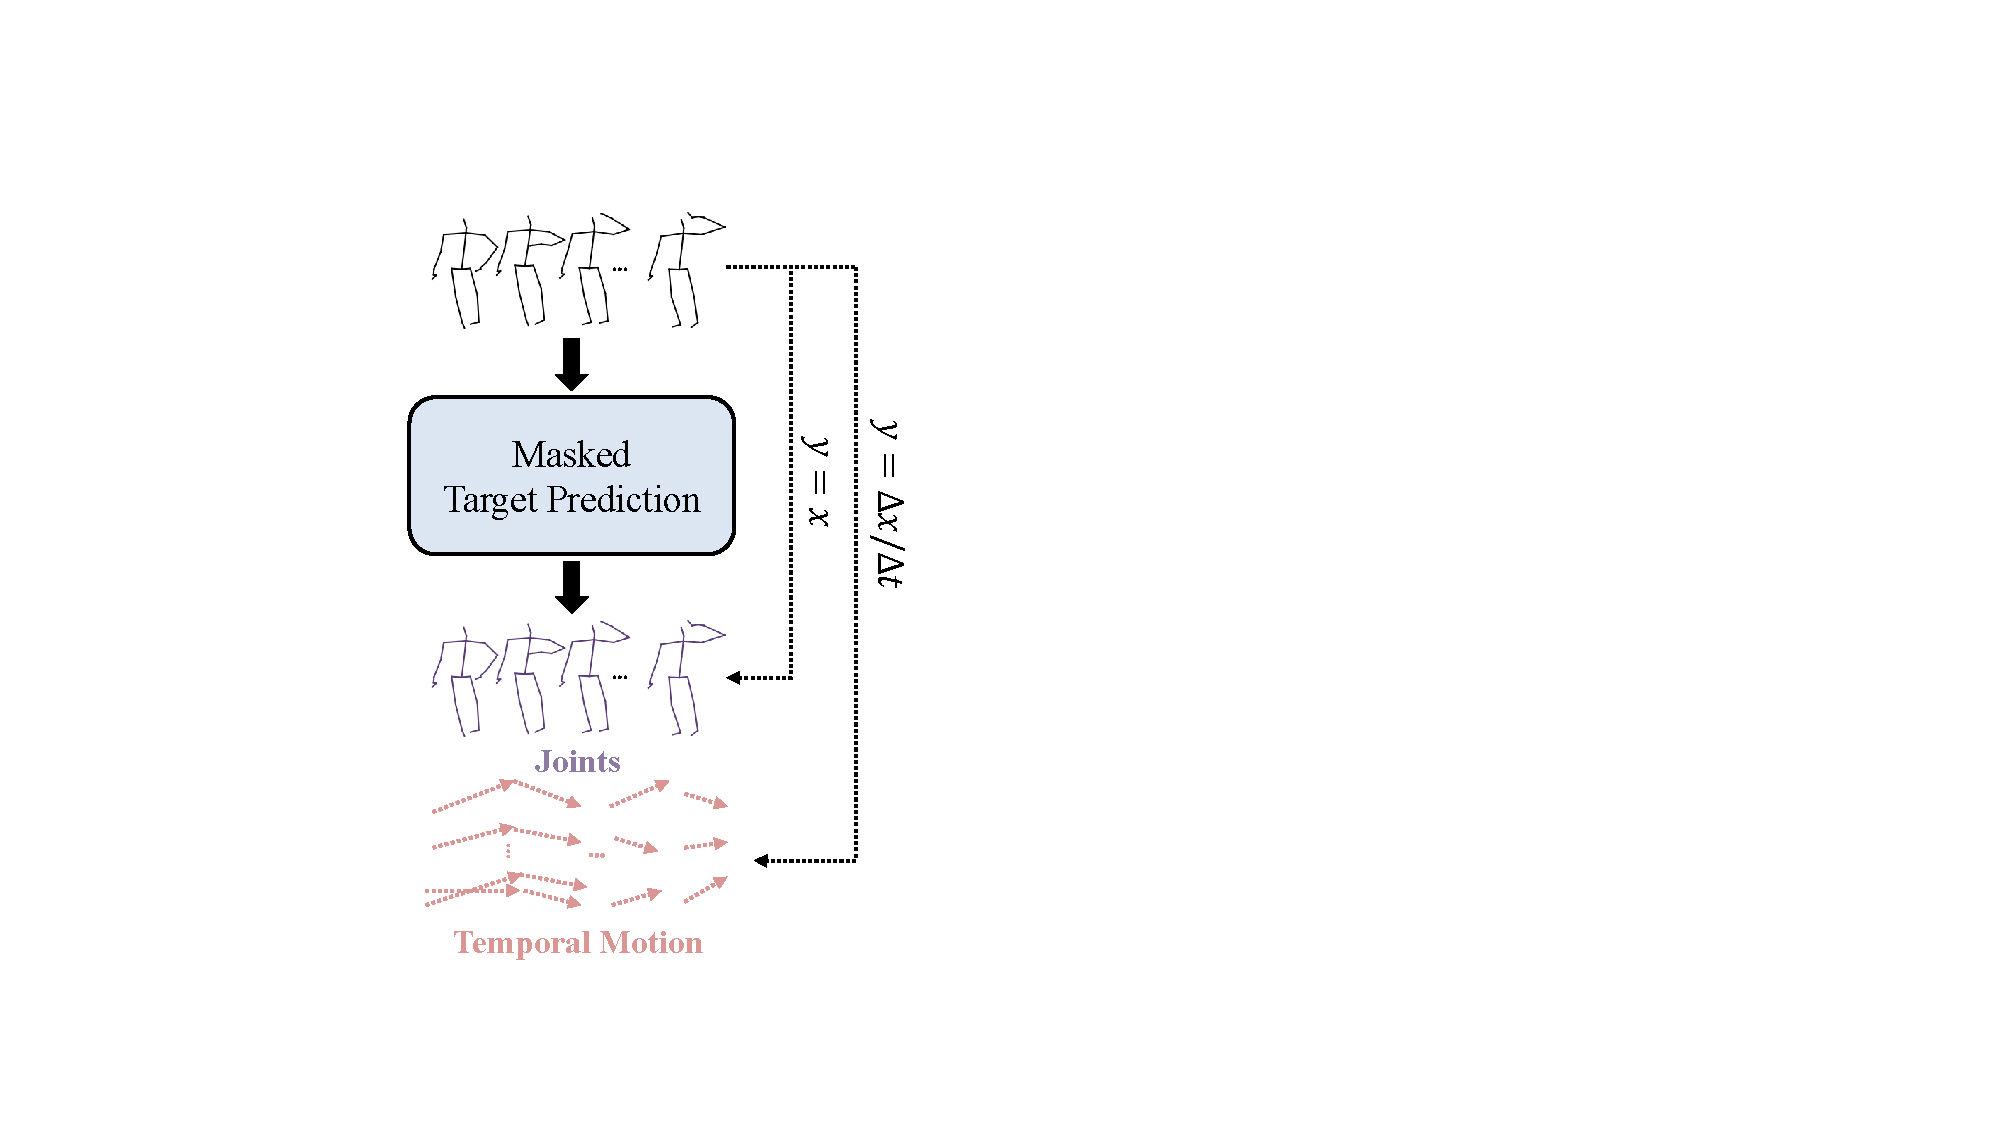
\includegraphics[width=0.5\linewidth]{figures/fig1_MAE.pdf}
% 		\caption{MAE-like}
% 		\label{fig1:MAE}
% 	\end{subfigure}
% 	\centering
% 	\begin{subfigure}{0.49\linewidth}
% 		\centering
% 		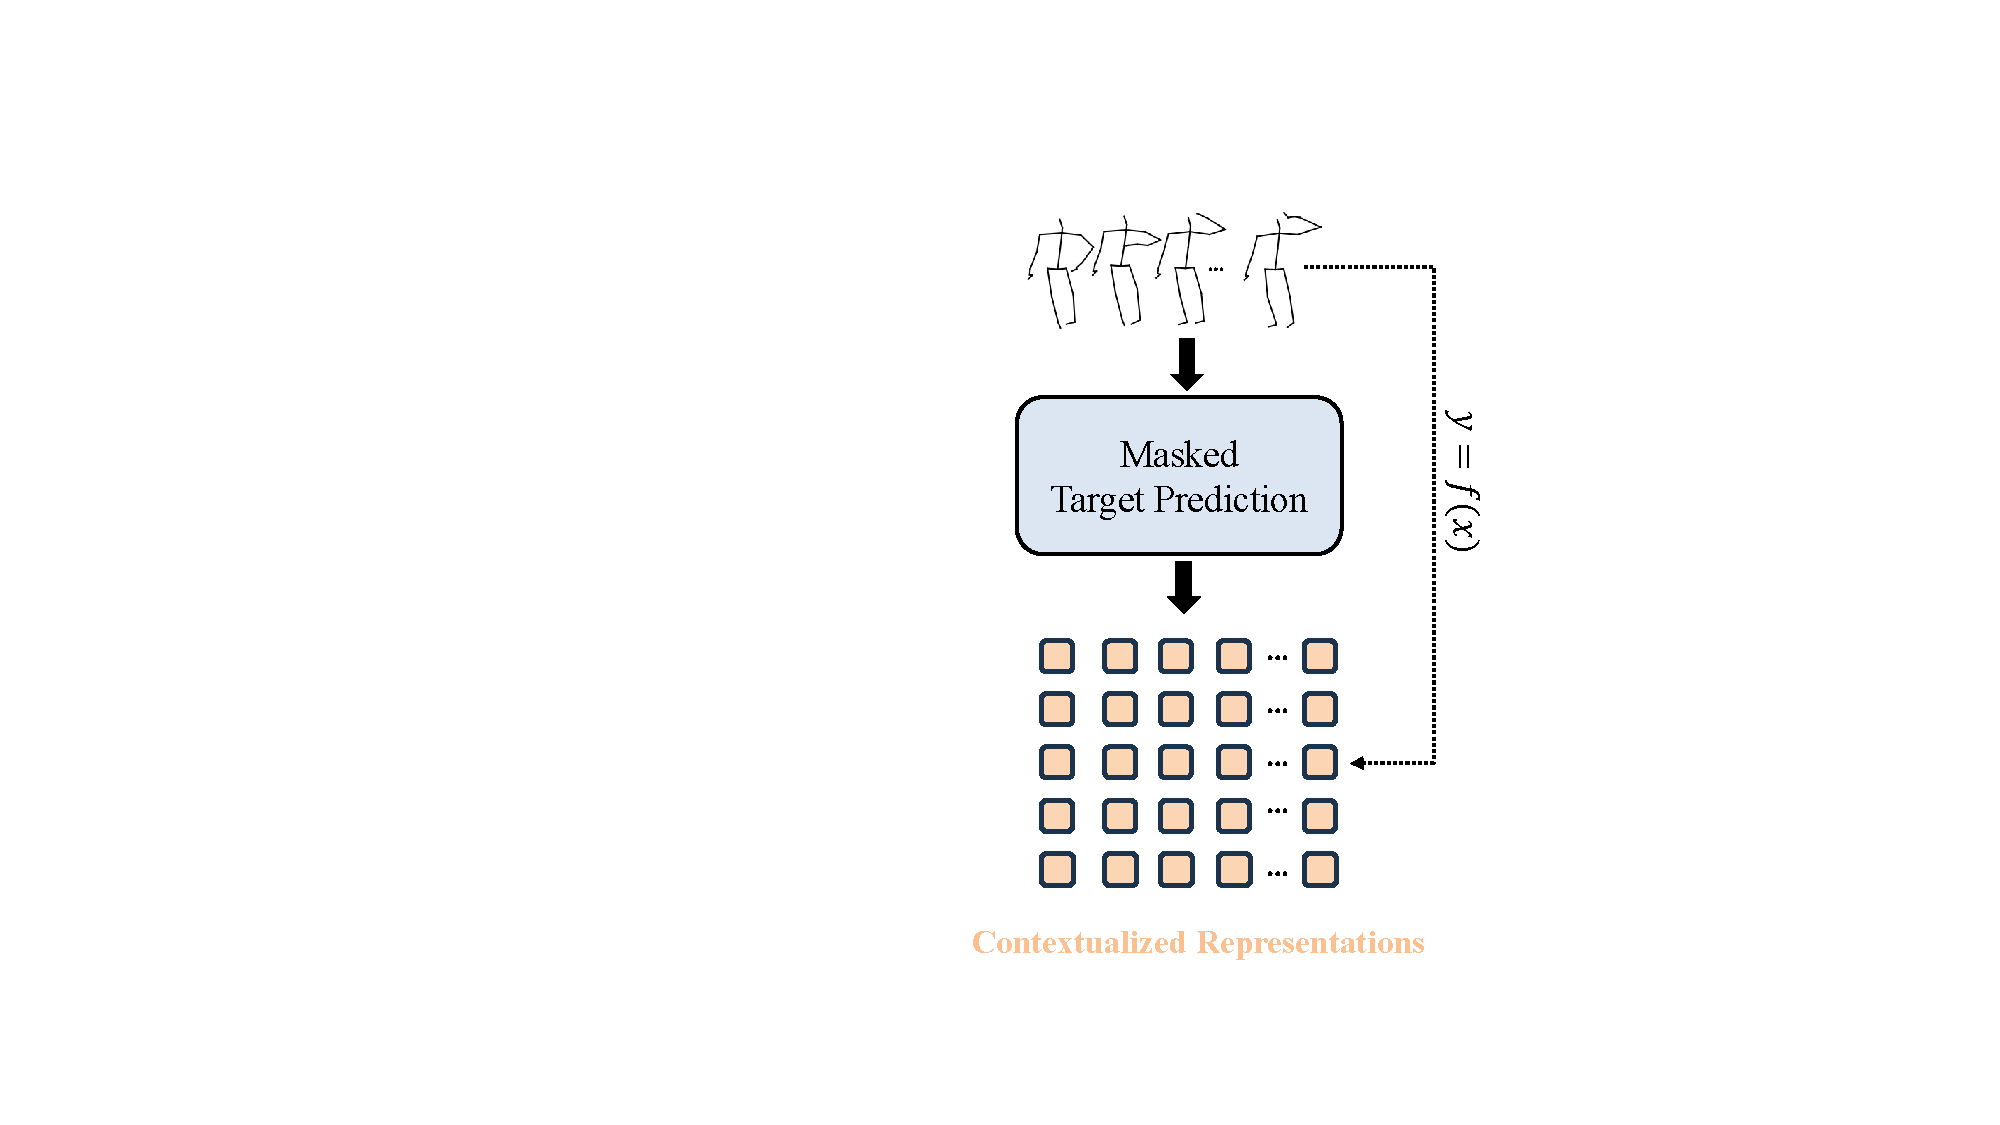
\includegraphics[width=0.5\linewidth]{figures/fig1_skeleton2vec.pdf}
% 		\caption{Skeleton2vec(Ours)}
% 		\label{fig1:skeleton2vec}
% 	\end{subfigure}
%     \caption{
%     A comparative illustration of the prediction targets between MAE-like methods (a) and
%     ours Skeleton2vec (b). Skeleton2vec utilizes an teacher encoder $f(x)$ to generate
%     globally contextualized representations as the prediction targets, instead of
%     isolated joints or temporal motion with only local context.
%     }
%     \label{fig1}
% \end{figure}

\begin{figure}
  \centering
  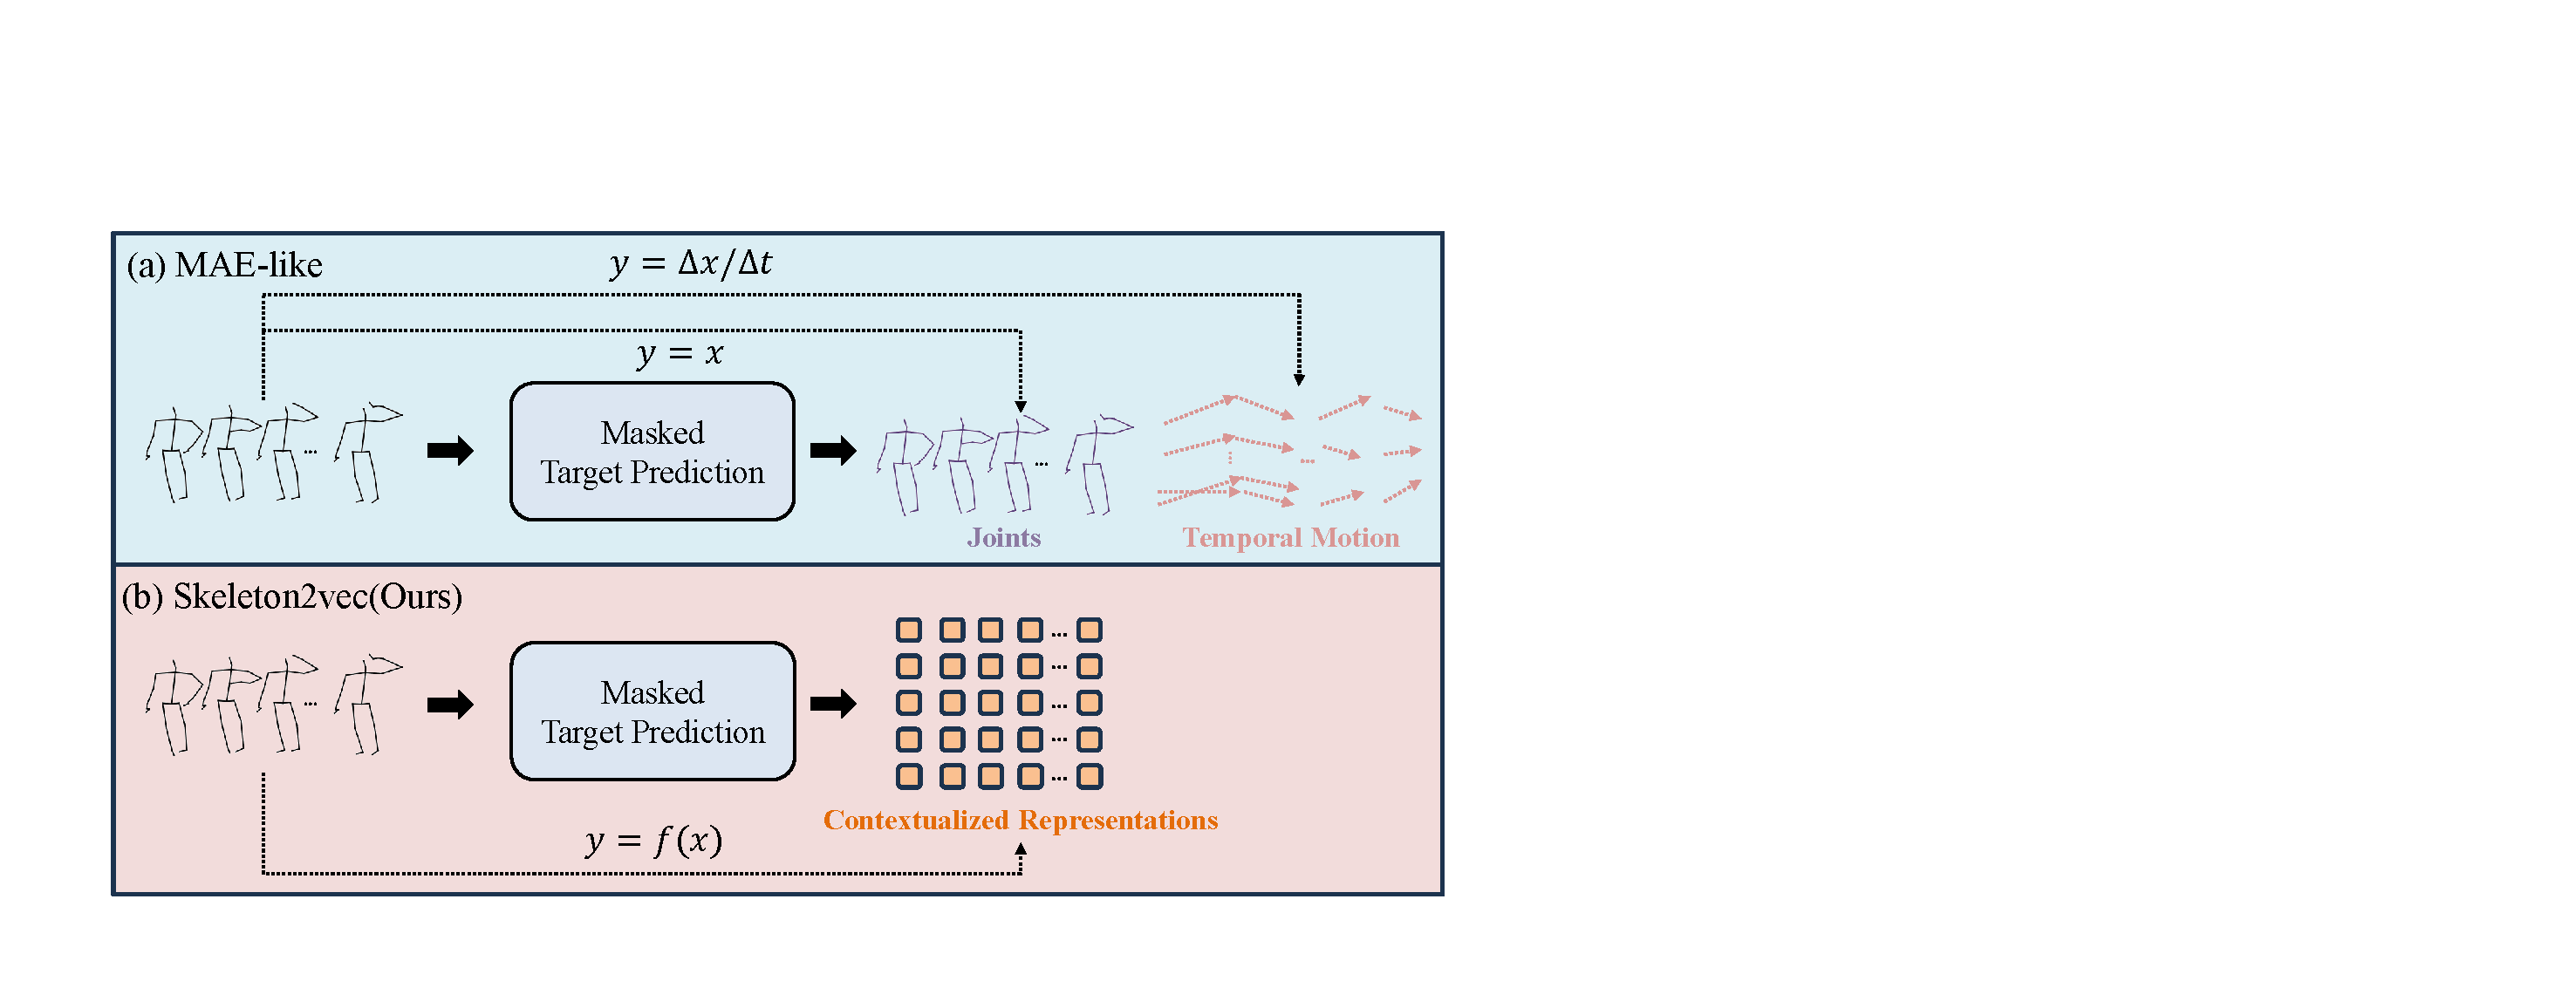
\includegraphics[width=0.80\linewidth]{figures/fig_mae_and_skeleton2vec.pdf}
    \caption{
    A comparative illustration of the prediction targets between MAE-like methods (a) and
    ours Skeleton2vec (b). Skeleton2vec utilizes an teacher encoder $f(x)$ to generate
    globally contextualized representations as the prediction targets, instead of
    isolated joints or temporal motion with only local context.
    }
    \label{fig1}
    \vspace{-15pt}
\end{figure}

Human action recognition has significant applications in the real world, such as
security, human-robot interaction, and virtual reality. The development of depth
sensors and advancements in pose estimation algorithms \cite{2018OpenPose, fang2017rmpe, xu2020deep}
have propelled skeleton-based action recognition into a popular research topic,
owing to its computational efficiency, background robustness, and privacy preservation.
A series of fully-supervised skeleton-based human action recognition methods have
been developed using CNNs \cite{du2015skeleton,li2017skeleton}, RNNs \cite{liu2016spatio,zhang2017view},
and GCNs \cite{yan2018spatial,chen2021channel}. Despite their promising performance,
these methods rely on large amounts of manually annotated data, which is expensive,
labor-intensive, and time-consuming to obtain. This circumstance motivates us
to explore self-supervised representation learning for 3D actions.

Earlier works \cite{lin2020ms2l, nie2020unsupervised, su2020predict, zheng2018unsupervised}
have employed various pretext tasks, such as motion prediction, jigsaw puzzle recognition,
and masked reconstruction, to learn 3D action representations. Recently, contrastive
learning methods \cite{rao2021augmented, guo2022contrastive, moliner2022bootstrapped, lin2023actionlet}
have gained prominence. However, these methods often require carefully designed
data augmentations and tend to encourage the encoder to learn more global
representations, thereby neglecting local spatiotemporal information.
With the rise of transformer models \cite{vaswani2017attention}, self-supervised
pre-training methods based on masked prediction tasks have become mainstream in
visual representation learning \cite{rao2021augmented, guo2022contrastive, moliner2022bootstrapped, lin2023actionlet}.
Works like SkeletonMAE \cite{yan2023skeletonmae, wu2023skeletonmae} and MAMP \cite{mao2023masked} have
attempted to transfer MAE \cite{he2022masked} methods to the field of 3D action representation
learning, achieving promising results. However, these MAE-like methods inefficiently
utilize model capacity by focusing on low-level high-frequency details with
raw joint coordinates or temporal motion as learning targets, which is suboptimal
for modeling high-level spatiotemporal structures. We believe that using
higher-level prediction targets will guide the model to learn better representations
and improve pre-training performance.

Motivated by this idea, we propose Skeleton2vec, a simple and efficient self-supervised
framework for 3D action representation learning. Addressing the limitations of existing
MAE-like methods, as illustrated in \cref{fig1}, Skeleton2vec leverages contextualized
prediction targets. Following the work of data2vec \cite{baevski2022data2vec, baevski2023efficient},
we employ a teacher encoder that takes unmasked training samples to generate latent
contextualized representations as targets. We then use a student encoder, taking a
masked version of the sample as input, combined with an asymmetric decoder to
predict data representations at the masked positions. The entire model is based on the
vanilla transformer architecture. The self-attention mechanism ensures that the
constructed targets are contextualized, incorporating information from the entire
sample, making them richer than isolated targets (\eg raw joint coordinates)
or targets based on local context (\eg temporal motion).

Additionally, considering the strong spatiotemporal correlations in 3D skeleton sequences,
we propose a Motion-Aware Multi-Tube (MAMT) masking strategy. Initially, we divide the input skeleton
sequence along the temporal axis into multiple tubes, where frames within each tube share
a masking map to avoid information leakage from neighboring frames. This forces the model to
extract information from distant time steps for better prediction. We then guide the sampling
of masked joints based on the spatial motion intensity of body joints within each tube.
Joints with higher motion intensity will be masked with higher probability, allowing
the model to focus more on spatiotemporal regions with rich action semantics. Compared
to random masking, our method better utilizes the spatiotemporal characteristics and
motion priors of 3D skeleton sequences, effectively improving pre-training performance.

In summary, the main contributions of this work are three-fold:
\begin{itemize}
    \item{
        We propose the Skeleton2vec framework, which uses contextualized representations
        from a teacher encoder as prediction targets, enabling the learned representations
        to have stronger semantic associations.
    }
    \item{
        We introduce a motion-aware multi-tube masking strategy that performs persistent masking
        of joints within tubes based on spatial motion intensity, forcing the model to
        build better long-range spatiotemporal connections and focus on more semantic-rich regions.
    }
    \item{
        We validate the effectiveness of our method on three large-scale 3D skeleton-based
        action recognition datasets and achieve state-of-the-art results.
    }
\end{itemize}